\documentclass[10pt]{article}

\usepackage[latin1]{inputenc}
\usepackage{amsmath, amssymb, amsfonts, amsthm}
\usepackage{upgreek}
\usepackage{amsthm}
\usepackage{fullpage}
\usepackage{graphicx}
\usepackage{cancel}
\usepackage{subfigure}
\usepackage{mathrsfs}
\usepackage{outlines}
\usepackage[font={sf,it}, labelfont={sf,bf}, labelsep=space, belowskip=5pt]{caption}
\usepackage{hyperref}
\usepackage{minted}
\usepackage{titling}

\usepackage{fancyhdr}
\usepackage[title]{appendix}

\DeclareMathOperator{\sgn}{sgn}

\pagestyle{fancy}
\headheight 24pt
\headsep    12pt
\lhead{Material Property Design}
\rhead{\today}
\fancyfoot[C]{} % hide the default page number at the bottom
\lfoot{}
\rfoot{\thepage}
\renewcommand{\headrulewidth}{0.4pt}
\renewcommand\footrulewidth{0.4pt}
\providecommand{\abs}[1]{\lvert#1\rvert}
\providecommand{\norm}[1]{\lVert#1\rVert}
\providecommand{\dx}{\, \mathrm{d}x}
% \providecommand{\vint}[2]{\int_{#1} \! #2 \, \mathrm{d}x}
% \providecommand{\sint}[2]{\int_{\partial #1} \! #2 \, \mathrm{d}A}
\renewcommand{\div}{\nabla \cdot}
\providecommand{\shape}{\Omega(p)}
\providecommand{\mesh}{\mathcal{M}}
\providecommand{\boundary}{\partial \shape}
\providecommand{\vint}[1]{\int_{\shape} \! #1 \, \mathrm{d}x}
\providecommand{\sint}[1]{\int_{\boundary} \! #1 \, \mathrm{d}A}
\providecommand{\pder}[2]{\frac{\partial #1}{\partial #2}}
\providecommand{\tder}[2]{\frac{\mathrm{d} #1}{\mathrm{d} #2}}
\providecommand{\evalat}[2]{\left.#1\right|_{#2}}
\newcommand{\defeq}{\vcentcolon=}
\newtheorem{lemma}{Lemma}

\makeatletter
\usepackage{mathtools}
\newcases{mycases}{\quad}{%
  \hfil$\m@th\displaystyle{##}$}{$\m@th\displaystyle{##}$\hfil}{\lbrace}{.}
\makeatother

\setlength{\droptitle}{-50pt}
\title{Approach to Material Property Design}
\author{}
% Move date up over where author would be...
\date{\vspace{-24pt} \today}

% BEGIN DOCUMENT
\begin{document}
\maketitle
We outline the basic approach and tools needed to achieve spatially varying
material properties on a single material printer via periodic, patterned
microstructures. We assume for now that we are given a coarse volume mesh,
$\mesh_c$, and that each element has been assigned an elasticity tensor or
material parameters. Ideally, each of these tensors lies in the space of
homogenized tensors spanned by our chosen patterns (this could be enforced by
the tool/optimization used to assign material properties). Our goal is to create
a fine-scale volume mesh, $\mesh_f$, filled with the printer's single,
homogeneous material so that the homogenized behavior of $\mesh_f \cap e$
approximates $e$'s input elasticity tensor for all coarse volume elements $e \in
\mesh_c$.
\section{Overview}
 The general approach is as follows:
\begin{enumerate}
    \setcounter{enumi}{-1}
    \item Read in the target material properties, $m_e$, for each $e \in
        \mesh_c$. These could be in the form of
        \label{step:read}
        \begin{enumerate}
            \item ``painted'' elasticity tensors from a library we know our
                patterns can approximate;
            \item elasticity tensors fit to object deformation measurements (e.g.
                  Matusik's ``shoe paper'', \cite{Bickel2010}); or
            \item elasticity tensors optimizing some objective (minimum
                  compliance, desired deformation, desired force
                  feedback).
        \end{enumerate}
    \item Fit pattern parameters. For each element $e \in \mesh_c$, invert the
        pattern parameters $\to$ material properties map to find parameters,
        $p_e$, for the periodic pattern closest to achieving the desired
        properties.
        \label{step:fit}
        \begin{enumerate}
            \item Use a precomputed pattern parameter to material properties
                lookup table built for our patterns to interpolate an
                approximate inverse. This table could be built by sampling an
                ``$\epsilon \to 0$'' formula, e.g. for sequential laminates
                \cite{allaire2002shape}, or by numerical homogenization \`a la
                \cite{Kharevych2009}.
            \item If we have an explicit ``$\epsilon \to 0$'' formula, run some
                iterations of Newton's method to improve the inverse.
        \end{enumerate}
        Notice that here we are taking advantage of Theorem 2.1.2 from
        \cite{allaire2002shape} to work pointwise; it says that a homogenized
        material field is valid/achievable if and only if its tensor value at
        every point is an elasticity tensor obtained by periodic homogenization.
    \item Generate a printable, fine-scale mesh, $\mesh_f$. Because patterns
        need to ``connect'' across coarse element boundaries, we cannot operate
        on each coarse element in isolation.
        \label{step:mesh}
        \begin{enumerate}
            \item Choose a length scale, $\epsilon$, (periodic cell size) based
                on printer resolution and printability concerns (thin features,
                etc.).
            \item Subdivide each $e \in \mesh_c$ into cells of this size,
                filling each with a mesh of the periodic pattern specified by
                $p_e$.
            \item Stitch together the microstructure cell meshes (see Section
                \ref{sec:gen_connect}).
        \end{enumerate}
    \item Fabricate $\mesh_f$.
    \label{step:fabricate}
\end{enumerate}

\section{Validation}
Each stage of the pipeline will introduce errors, and it will be important to
measure these errors individually.

From this write-up's perspective, step \ref{step:read} gives the ground truth:
the final, fabricated object better behave like a FEM simulation of $\mesh_c$.
However, if/when the scope of our project expands to include
compliance/deformation optimization or object duplication, we will need to see
how much this simulation differs from the desired result.

Step \ref{step:fit}'s error can be measured accurately if we have a formula
that maps pattern parameters to homogenized material properties. For the class
of sequential laminates, we have just that: e.g. (2.67) and (2.151) in
\cite{allaire2002shape}. However, if we instead only have a lookup table,
measuring the error is impossible; we do not know the material properties
corresponding to our interpolated guess of pattern parameters. Worse, if our
desired material properties are far from the entries in the lookup table, we do
not know if that is because the lookup table is incomplete or the material is
not achievable.

Steps \ref{step:fit}-\ref{step:mesh} can be tested by comparing a simulation of
$\mesh_f$ with the simulation of $\mesh_c$. Unfortunately, step \ref{step:mesh}
accumulates two errors that are hard to separate. The first is the failure of
the finite-sized pattern to match its homogenized tensor. If the pattern is one
we homogenized by the ``$\epsilon \to 0$'', mathematical approach
\cite{allaire2002shape}, then error arises from the fact $\epsilon > 0$. If
instead the pattern was homogenized by something akin to \cite{Kharevych2009},
the error is due to the inaccuracy in the numerical coarsening itself. The
second type of error is in how the cells connect. Theorem 2.1.2 of
\cite{allaire2002shape} that allows us to assign periodically homogenized
elasticity tensors pointwise is only valid in the limit as the periodic cell
shrinks to zero. It does not tell us how to connect finite-sized cells or even
say that it is possible. This stitching will be one of the key challenges
(Section \ref{sec:gen_connect}).

Step \ref{step:fabricate} introduces another, probably quite large error: unpredictable
variations in the 3D printer's material properties. Unfortunately, there's not
much we can do here. Hopefully the error will be small enough that we can still
make qualitative comparisons to the ground-truth simulation of $\mesh_c$ and
only present quantitative comparisons in the evaluation of $\mesh_f$ (step
\ref{step:mesh}).

\subsection{Test Cases}
\begin{itemize}
    \item Rectangular bar of isotropic material with Young's modulus varying from one end
        to the other.
    \item Rectangular bar of orthotropic material with material axis rotating
        from one end to the other.
\end{itemize}

\section{Generating/Connecting the Microstructures}
\label{sec:gen_connect}
One of the greatest challenges is connecting the microstructures generated for
each element in $\mesh_c$ into a single fine microstructure mesh, $\mesh_f$. We
will likely consider periodic patterns that tile perfectly, but since elements
are to be filled with different patterns, there are no guarantees that patterns
will match up across internal faces of $\mesh_c$.

We will need to think a lot on this, but here is one possible starting
direction. Assume $\mesh_c$ is a cube voxel grid. Then, by choosing $\epsilon$
to be a divisor of this grid size, we can easily subdivide the grid into fine
cubic cells as mentioned in step \ref{step:mesh} and fill each with its coarse
element's pattern. Then, inside each $e \in \mesh_c$ the tiling is perfect
(assuming periodic patterns). If we make the further assumption that the
patterns' boundary shapes are continuous functions of their parameters, then
cells will nearly connect with their neighbors when those neighbors' pattern
parameters are similar. So, as long as there are no sharp jumps in pattern
parameters, it should be possible to warp these transition boundaries to connect
seamlessly with each other. We could ensure this by smoothing the pattern
parameter quantities near the problematic transitions either with interpolation
or solving a Laplace equation with appropriate boundary conditions.

Another approach is specific to the sequential laminate patterns, for which the
parameters are the material proportions and orientations for each of the $p$
lamination directions. We could fit smooth lamination direction curves to the
direction vectors sitting on each element $e \in \mesh_c$. There will be at
least $3$ of these vectors in arbitrary (non-orthogonal) orientation, but
hopefully the directions will vary smooth enough that registering them between
adjacent elements is possible. These lamination direction curves specify the
line orthogonal to which thin planar slices of the material should be added with
density given by that direction line's (interpolated) proportion. These planar
slices intersect to form a deformed lattice structure (or, if you prefer, a
matrix of polyhedral void regions). The size of these planes is not immediately
clear, nor is how they will intersect with neighboring coarse elements' planes.

\section{Circumventing ``Stitching'' Patterns}
\label{sec:procedual_pattern}
In general, the desired material tensor field (output of step 0) is a smooth
function over the domain.  We can approximate this field either by an
element-wise constant field, which is the approached assumed in Section
\ref{sec:gen_connect}, or by an element-wise tri-linear field.  The first
approach would introduce sharp discontinuities around element boundaries, thus
the need to stitch the microstructure from neighbor elements together.
On the other hand, the second approach does not have such discontinuities since
element-wise tri-linear field is continous.

The difficulty of having an element-wise tri-linear material tensor field is
that it is not clear how to ``tile'' patterns.  In the setting of sequantial
laminates, there are at least two ways of doing this.  Both approaches generate
a mesh that is locally made of sequantial laminates almost everywhere.

\subsection{Laminate tracing}
It is common in visualization to trace streamlines according to a vector field.
In particular, the streamline direction accurately represents the vector
directions at each point in the domain.  For sequential laminates of rank $p$, we have
$p$ layers of lamination, where for each layer the pattern parameters consist of
a lamination direction and a material ratio, both are smooth fields over the
domain.  This
allows us to trace out each laminate slice one by one, where the thickness of
the slice remains constant and the density of the laminates (how closely packed one
slice is from another slice) is determined by the material ratio.

\begin{figure}[t]
\centering
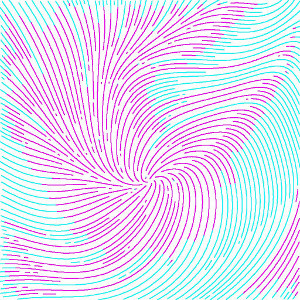
\includegraphics[height=0.3\textwidth]{images/streamlines}
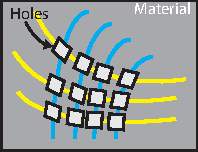
\includegraphics[height=0.3\textwidth]{images/hole_packing}
\caption{Left: It is easy to trace streamlines from a given vector field.  The
density of the streamlines can be directly controled.
Right: The lamination directions can be traced.  They forms a set of
streamlines, where we can procedually insert holes at their intersetions.}
\label{fig:hole_packing}
\end{figure}

\subsection{Hole packing}
Hole packing is similar to laminate tracing, but perhaps easier to generate.  Sequential
laminates of rank $p$ (with $p\ge3$ in $\mathbb{R}^3$) have the property that it
partitions the domain into small disconnected voids.  (Let's ignore printability
for now.)  So instead of trying to lay out slices of laminates, one can
think in terms of where to place those holes.  The material parameters ($p$
lamination directions and $p$ material ratios) uniquely determine the shape of
the hole at each point up to scale.   We just need to know where to place those
holes such that the resulting microstructure is sequantial laminates.

The hole packing algorithm uses the streamlines traced along the lamination
directions (i.e. streamlines are orthogonal to each laminate slice).  Since
there are $p$ sets of streamlines, the stream lines form a grid (more precisely
a network).  In 2D, two
sets of non-parallel streamlines always intersect.  In 3D, since the material
property is a smooth field, we can generate sets of streamlines such that they
do intersect.  The hole packing algorithm put a hole whenever two stream
lines intersect. The shape of the hole is determined by the lamination
directions, and the size of the hole is determined by the local material ratios.
This approach is illustrated in Figure \ref{fig:hole_packing}.  The resulting
microstructure (the complement of the holes) is almost a sequential laminate
everywhere.  Only at locations where a streamline begins or ends, the
microstructure is locally different from sequential laminates.


\section{Printability}
Not only do we need to choose the periodic cell size large enough that the
printer can resolve the patterns' details without violating any design rules,
but also we must worry about internal voids in the case of the single material
application. In the single material case, the patterns comprise solid and void
regions (as opposed to solid regions of distinct materials for multi-material
printing). To allow support material removal, these voids must all have a path
to the object's exterior.

The printibility concerns could be avoided when printing with multi-material
printers, where one can replace void with a very weak material.

\section{Simulating and Meshing the Microstructure}
For simulation alone, it will probably be easiest to implement the composite
material as an inside/outside indicator function and run the CSGFEM meshfree
implementation. This prevents us from having to mesh the geometry and should be
reasonably accurate, provided we refine the computation grid enough.

However, for printing we probably need an actual mesh. The procedure chosen for
generating and connecting patterns (Section \ref{sec:gen_connect}) must be
extended to stitch meshes together. E.g., for the general periodic pattern
connection approach described in Section \ref{sec:gen_connect}, identically
patterned neighboring cells can be stitched together trivially, and those with
similar boundary shapes could be stitched together after warping, assuming
consistent boundary meshing.

\section{Search for Patterns}
As described above, it will be desirable to have periodic patterns that are
parametrized smoothly. Ideally these patterns will also have an analytic formula
for their homogenized elasticity tensors/material properties,
but we may be able to get away with the numerical coarsening +
look-up-table-only fitting approach.

Even more importantly, the pattern we choose must have good coverage of the
range of desired material properties. We discuss this in the next section.

\section{Toward a Proof of Concept}
The most important experiment that we can run now is to test that we can achieve
a useful range of material properties with a single material printer. The best
tool we have for this is currently the sequential laminate
\cite{allaire2002shape}. This is a pattern for which several closed formulas
exist for homogenized elasticity tensors. Perhaps other patterns can achieve a
wider range of materials, but we would need to develop our own machinery to
analyze them.

So far we have looked only at the space of approximately isotropic homogenized
tensors achieved by rank $1, 2, $ and $3$ sequential laminates of two
non-void, isotropic materials. Though we have not analyzed all our data, we
found that the laminates were roughly able to interpolate between the two
materials' Young's moduli (Poisson ratio remained mostly unchanged). It will be
important to look also at the space of orthotropic materials. We also need to
consider the case were one material is void (Section 2.3.4 of
\cite{allaire2002shape}).


\section{Miscellaneous Concerns}
\begin{itemize}
    \item The homogenization theory is built around linear elasticity. If we want to
        design large-scale deformation behavior, we will probably have to
        consider a non-linear version (if possible).

    \item What material will be used to coat the object? It is likely that
        printing the skin will introduce rigidity that prevents all the
        deformation behavior our internal microstructures are designed to
        support.
\end{itemize}

\bibliographystyle{plain}
\bibliography{References}

\end{document}

